\documentclass[1p]{elsarticle_modified}
%\bibliographystyle{elsarticle-num}

%\usepackage[colorlinks]{hyperref}
%\usepackage{abbrmath_seonhwa} %\Abb, \Ascr, \Acal ,\Abf, \Afrak
\usepackage{amsfonts}
\usepackage{amssymb}
\usepackage{amsmath}
\usepackage{amsthm}
\usepackage{scalefnt}
\usepackage{amsbsy}
\usepackage{kotex}
\usepackage{caption}
\usepackage{subfig}
\usepackage{color}
\usepackage{graphicx}
\usepackage{xcolor} %% white, black, red, green, blue, cyan, magenta, yellow
\usepackage{float}
\usepackage{setspace}
\usepackage{hyperref}

\usepackage{tikz}
\usetikzlibrary{arrows}

\usepackage{multirow}
\usepackage{array} % fixed length table
\usepackage{hhline}

%%%%%%%%%%%%%%%%%%%%%
\makeatletter
\renewcommand*\env@matrix[1][\arraystretch]{%
	\edef\arraystretch{#1}%
	\hskip -\arraycolsep
	\let\@ifnextchar\new@ifnextchar
	\array{*\c@MaxMatrixCols c}}
\makeatother %https://tex.stackexchange.com/questions/14071/how-can-i-increase-the-line-spacing-in-a-matrix
%%%%%%%%%%%%%%%

\usepackage[normalem]{ulem}

\newcommand{\msout}[1]{\ifmmode\text{\sout{\ensuremath{#1}}}\else\sout{#1}\fi}
%SOURCE: \msout is \stkout macro in https://tex.stackexchange.com/questions/20609/strikeout-in-math-mode

\newcommand{\cancel}[1]{
	\ifmmode
	{\color{red}\msout{#1}}
	\else
	{\color{red}\sout{#1}}
	\fi
}

\newcommand{\add}[1]{
	{\color{blue}\uwave{#1}}
}

\newcommand{\replace}[2]{
	\ifmmode
	{\color{red}\msout{#1}}{\color{blue}\uwave{#2}}
	\else
	{\color{red}\sout{#1}}{\color{blue}\uwave{#2}}
	\fi
}

\newcommand{\Sol}{\mathcal{S}} %segment
\newcommand{\D}{D} %diagram
\newcommand{\A}{\mathcal{A}} %arc


%%%%%%%%%%%%%%%%%%%%%%%%%%%%%5 test

\def\sl{\operatorname{\textup{SL}}(2,\Cbb)}
\def\psl{\operatorname{\textup{PSL}}(2,\Cbb)}
\def\quan{\mkern 1mu \triangleright \mkern 1mu}

\theoremstyle{definition}
\newtheorem{thm}{Theorem}[section]
\newtheorem{prop}[thm]{Proposition}
\newtheorem{lem}[thm]{Lemma}
\newtheorem{ques}[thm]{Question}
\newtheorem{cor}[thm]{Corollary}
\newtheorem{defn}[thm]{Definition}
\newtheorem{exam}[thm]{Example}
\newtheorem{rmk}[thm]{Remark}
\newtheorem{alg}[thm]{Algorithm}

\newcommand{\I}{\sqrt{-1}}
\begin{document}

%\begin{frontmatter}
%
%\title{Boundary parabolic representations of knots up to 8 crossings}
%
%%% Group authors per affiliation:
%\author{Yunhi Cho} 
%\address{Department of Mathematics, University of Seoul, Seoul, Korea}
%\ead{yhcho@uos.ac.kr}
%
%
%\author{Seonhwa Kim} %\fnref{s_kim}}
%\address{Center for Geometry and Physics, Institute for Basic Science, Pohang, 37673, Korea}
%\ead{ryeona17@ibs.re.kr}
%
%\author{Hyuk Kim}
%\address{Department of Mathematical Sciences, Seoul National University, Seoul 08826, Korea}
%\ead{hyukkim@snu.ac.kr}
%
%\author{Seokbeom Yoon}
%\address{Department of Mathematical Sciences, Seoul National University, Seoul, 08826,  Korea}
%\ead{sbyoon15@snu.ac.kr}
%
%\begin{abstract}
%We find all boundary parabolic representation of knots up to 8 crossings.
%
%\end{abstract}
%\begin{keyword}
%    \MSC[2010] 57M25 
%\end{keyword}
%
%\end{frontmatter}

%\linenumbers
%\tableofcontents
%
\newcommand\colored[1]{\textcolor{white}{\rule[-0.35ex]{0.8em}{1.4ex}}\kern-0.8em\color{red} #1}%
%\newcommand\colored[1]{\textcolor{white}{ #1}\kern-2.17ex	\textcolor{white}{ #1}\kern-1.81ex	\textcolor{white}{ #1}\kern-2.15ex\color{red}#1	}

{\Large $\underline{12n_{0407}~(K12n_{0407})}$}

\setlength{\tabcolsep}{10pt}
\renewcommand{\arraystretch}{1.6}
\vspace{1cm}\begin{tabular}{m{100pt}>{\centering\arraybackslash}m{274pt}}
\multirow{5}{120pt}{
	\centering
	\includegraphics[width=112pt]{../../../GIT/diagram.site/Diagrams/png/2496_12n_0407.png}\\
\ \ \ A knot diagram\footnotemark}&
\allowdisplaybreaks
\textbf{Linearized knot diagam} \\
\cline{2-2}
 &
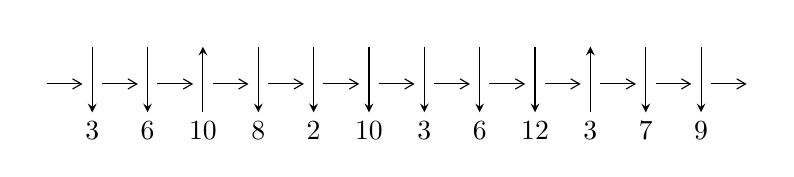
\begin{tikzpicture}[x=20pt, y=17pt]
	% nodes
	\node (C0) at (0, 0) {};
	\node (C1) at (1, 0) {};
	\node (C1U) at (1, +1) {};
	\node (C1D) at (1, -1) {3};

	\node (C2) at (2, 0) {};
	\node (C2U) at (2, +1) {};
	\node (C2D) at (2, -1) {6};

	\node (C3) at (3, 0) {};
	\node (C3U) at (3, +1) {};
	\node (C3D) at (3, -1) {10};

	\node (C4) at (4, 0) {};
	\node (C4U) at (4, +1) {};
	\node (C4D) at (4, -1) {8};

	\node (C5) at (5, 0) {};
	\node (C5U) at (5, +1) {};
	\node (C5D) at (5, -1) {2};

	\node (C6) at (6, 0) {};
	\node (C6U) at (6, +1) {};
	\node (C6D) at (6, -1) {10};

	\node (C7) at (7, 0) {};
	\node (C7U) at (7, +1) {};
	\node (C7D) at (7, -1) {3};

	\node (C8) at (8, 0) {};
	\node (C8U) at (8, +1) {};
	\node (C8D) at (8, -1) {6};

	\node (C9) at (9, 0) {};
	\node (C9U) at (9, +1) {};
	\node (C9D) at (9, -1) {12};

	\node (C10) at (10, 0) {};
	\node (C10U) at (10, +1) {};
	\node (C10D) at (10, -1) {3};

	\node (C11) at (11, 0) {};
	\node (C11U) at (11, +1) {};
	\node (C11D) at (11, -1) {7};

	\node (C12) at (12, 0) {};
	\node (C12U) at (12, +1) {};
	\node (C12D) at (12, -1) {9};
	\node (C13) at (13, 0) {};

	% arrows
	\draw[->,>={angle 60}]
	(C0) edge (C1) (C1) edge (C2) (C2) edge (C3) (C3) edge (C4) (C4) edge (C5) (C5) edge (C6) (C6) edge (C7) (C7) edge (C8) (C8) edge (C9) (C9) edge (C10) (C10) edge (C11) (C11) edge (C12) (C12) edge (C13) ;	\draw[->,>=stealth]
	(C1U) edge (C1D) (C2U) edge (C2D) (C3D) edge (C3U) (C4U) edge (C4D) (C5U) edge (C5D) (C6U) edge (C6D) (C7U) edge (C7D) (C8U) edge (C8D) (C9U) edge (C9D) (C10D) edge (C10U) (C11U) edge (C11D) (C12U) edge (C12D) ;
	\end{tikzpicture} \\
\hhline{~~} \\& 
\textbf{Solving Sequence} \\ \cline{2-2} 
 &
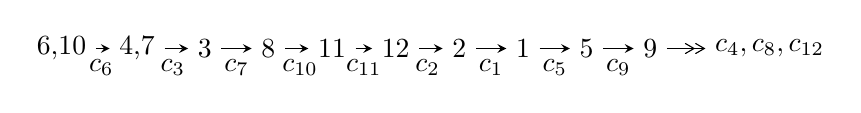
\begin{tikzpicture}[x=23pt, y=7pt]
	% node
	\node (A0) at (-1/8, 0) {6,10};
	\node (A1) at (17/16, 0) {4,7};
	\node (A2) at (17/8, 0) {3};
	\node (A3) at (25/8, 0) {8};
	\node (A4) at (33/8, 0) {11};
	\node (A5) at (41/8, 0) {12};
	\node (A6) at (49/8, 0) {2};
	\node (A7) at (57/8, 0) {1};
	\node (A8) at (65/8, 0) {5};
	\node (A9) at (73/8, 0) {9};
	\node (C1) at (1/2, -1) {$c_{6}$};
	\node (C2) at (13/8, -1) {$c_{3}$};
	\node (C3) at (21/8, -1) {$c_{7}$};
	\node (C4) at (29/8, -1) {$c_{10}$};
	\node (C5) at (37/8, -1) {$c_{11}$};
	\node (C6) at (45/8, -1) {$c_{2}$};
	\node (C7) at (53/8, -1) {$c_{1}$};
	\node (C8) at (61/8, -1) {$c_{5}$};
	\node (C9) at (69/8, -1) {$c_{9}$};
	\node (A10) at (11, 0) {$c_{4},c_{8},c_{12}$};

	% edge
	\draw[->,>=stealth]	
	(A0) edge (A1) (A1) edge (A2) (A2) edge (A3) (A3) edge (A4) (A4) edge (A5) (A5) edge (A6) (A6) edge (A7) (A7) edge (A8) (A8) edge (A9) ;
	\draw[->>,>={angle 60}]	
	(A9) edge (A10);
\end{tikzpicture} \\ 

\end{tabular} \\

\footnotetext{
The image of knot diagram is generated by the software ``\textbf{Draw programme}" developed by Andrew Bartholomew(\url{http://www.layer8.co.uk/maths/draw/index.htm\#Running-draw}), where we modified some parts for our purpose(\url{https://github.com/CATsTAILs/LinksPainter}).
}\phantom \\ \newline 
\centering \textbf{Ideals for irreducible components\footnotemark of $X_{\text{par}}$} 
 
\begin{align*}
I^u_{1}&=\langle 
-7.91368\times10^{38} u^{28}+9.57768\times10^{38} u^{27}+\cdots+2.45804\times10^{41} b+3.47957\times10^{40},\\
\phantom{I^u_{1}}&\phantom{= \langle  }2.07300\times10^{41} u^{28}-1.33160\times10^{41} u^{27}+\cdots+3.22003\times10^{43} a-6.95309\times10^{43},\\
\phantom{I^u_{1}}&\phantom{= \langle  }u^{29}- u^{28}+\cdots+138 u-131\rangle \\
I^u_{2}&=\langle 
107 u^{10}+32 u^9+296 u^8-244 u^7+366 u^6-671 u^5+173 u^4-379 u^3+801 u^2+137 b-343 u+11,\\
\phantom{I^u_{2}}&\phantom{= \langle  }-65 u^{10}-22 u^9-135 u^8+202 u^7-29 u^6+487 u^5+78 u^4+115 u^3-525 u^2+137 a+56 u+138,\\
\phantom{I^u_{2}}&\phantom{= \langle  }u^{11}+3 u^9-3 u^8+5 u^7-8 u^6+5 u^5-6 u^4+9 u^3-7 u^2+3 u-1\rangle \\
\\
\end{align*}
\raggedright * 2 irreducible components of $\dim_{\mathbb{C}}=0$, with total 40 representations.\\
\footnotetext{All coefficients of polynomials are rational numbers. But the coefficients are sometimes approximated in decimal forms when there is not enough margin.}
\newpage
\renewcommand{\arraystretch}{1}
\centering \section*{I. $I^u_{1}= \langle -7.91\times10^{38} u^{28}+9.58\times10^{38} u^{27}+\cdots+2.46\times10^{41} b+3.48\times10^{40},\;2.07\times10^{41} u^{28}-1.33\times10^{41} u^{27}+\cdots+3.22\times10^{43} a-6.95\times10^{43},\;u^{29}- u^{28}+\cdots+138 u-131 \rangle$}
\flushleft \textbf{(i) Arc colorings}\\
\begin{tabular}{m{7pt} m{180pt} m{7pt} m{180pt} }
\flushright $a_{6}=$&$\begin{pmatrix}1\\0\end{pmatrix}$ \\
\flushright $a_{10}=$&$\begin{pmatrix}0\\u\end{pmatrix}$ \\
\flushright $a_{4}=$&$\begin{pmatrix}-0.00643783 u^{28}+0.00413537 u^{27}+\cdots+0.662423 u+2.15933\\0.00321951 u^{28}-0.00389647 u^{27}+\cdots-1.02149 u-0.141559\end{pmatrix}$ \\
\flushright $a_{7}=$&$\begin{pmatrix}1\\u^2\end{pmatrix}$ \\
\flushright $a_{3}=$&$\begin{pmatrix}-0.00643783 u^{28}+0.00413537 u^{27}+\cdots+0.662423 u+2.15933\\0.000740929 u^{28}+0.00319203 u^{27}+\cdots-1.54711 u-0.443182\end{pmatrix}$ \\
\flushright $a_{8}=$&$\begin{pmatrix}-0.00128485 u^{28}+0.00710786 u^{27}+\cdots-1.02644 u+0.742688\\0.00237299 u^{28}+0.00288909 u^{27}+\cdots+0.812621 u-0.726496\end{pmatrix}$ \\
\flushright $a_{11}=$&$\begin{pmatrix}0.00280137 u^{28}-0.000100345 u^{27}+\cdots+5.91373 u-1.91339\\-0.00280112 u^{28}+0.00521011 u^{27}+\cdots+0.914236 u+0.185519\end{pmatrix}$ \\
\flushright $a_{12}=$&$\begin{pmatrix}-0.00302164 u^{28}+0.00557538 u^{27}+\cdots+4.99373 u-1.74508\\0.00526331 u^{28}-0.00557686 u^{27}+\cdots+0.171748 u+0.166224\end{pmatrix}$ \\
\flushright $a_{2}=$&$\begin{pmatrix}-0.00569690 u^{28}+0.00732739 u^{27}+\cdots-0.884682 u+1.71614\\0.000740929 u^{28}+0.00319203 u^{27}+\cdots-1.54711 u-0.443182\end{pmatrix}$ \\
\flushright $a_{1}=$&$\begin{pmatrix}0.00343665 u^{28}+0.00333715 u^{27}+\cdots-4.10542 u+1.78332\\0.000428392 u^{28}-0.00831580 u^{27}+\cdots-1.31725 u+0.269050\end{pmatrix}$ \\
\flushright $a_{5}=$&$\begin{pmatrix}-0.00619815 u^{28}+0.00185133 u^{27}+\cdots+1.94172 u+1.98378\\-0.00478198 u^{28}-0.00236596 u^{27}+\cdots-1.38469 u+1.09344\end{pmatrix}$ \\
\flushright $a_{9}=$&$\begin{pmatrix}-0.00365784 u^{28}+0.00421878 u^{27}+\cdots-1.83906 u+1.46918\\0.00237299 u^{28}+0.00288909 u^{27}+\cdots+0.812621 u-0.726496\end{pmatrix}$\\&\end{tabular}
\flushleft \textbf{(ii) Obstruction class $= -1$}\\~\\
\flushleft \textbf{(iii) Cusp Shapes $= -0.0105084 u^{28}+0.00112769 u^{27}+\cdots+16.0288 u-8.53764$}\\~\\
\newpage\renewcommand{\arraystretch}{1}
\flushleft \textbf{(iv) u-Polynomials at the component}\newline \\
\begin{tabular}{m{50pt}|m{274pt}}
Crossings & \hspace{64pt}u-Polynomials at each crossing \\
\hline $$\begin{aligned}c_{1}\end{aligned}$$&$\begin{aligned}
&u^{29}+36 u^{28}+\cdots+31 u+1
\end{aligned}$\\
\hline $$\begin{aligned}c_{2},c_{5}\end{aligned}$$&$\begin{aligned}
&u^{29}+4 u^{28}+\cdots- u+1
\end{aligned}$\\
\hline $$\begin{aligned}c_{3},c_{10}\end{aligned}$$&$\begin{aligned}
&u^{29}-2 u^{28}+\cdots+8 u+1
\end{aligned}$\\
\hline $$\begin{aligned}c_{4}\end{aligned}$$&$\begin{aligned}
&u^{29}+3 u^{28}+\cdots+365 u+41
\end{aligned}$\\
\hline $$\begin{aligned}c_{6}\end{aligned}$$&$\begin{aligned}
&u^{29}+u^{28}+\cdots+138 u+131
\end{aligned}$\\
\hline $$\begin{aligned}c_{7}\end{aligned}$$&$\begin{aligned}
&u^{29}- u^{28}+\cdots+19 u+1
\end{aligned}$\\
\hline $$\begin{aligned}c_{8}\end{aligned}$$&$\begin{aligned}
&u^{29}-6 u^{28}+\cdots-2946 u+449
\end{aligned}$\\
\hline $$\begin{aligned}c_{9},c_{12}\end{aligned}$$&$\begin{aligned}
&u^{29}-3 u^{28}+\cdots+4 u+1
\end{aligned}$\\
\hline $$\begin{aligned}c_{11}\end{aligned}$$&$\begin{aligned}
&u^{29}-2 u^{28}+\cdots+814 u+143
\end{aligned}$\\
\hline
\end{tabular}\\~\\
\newpage\renewcommand{\arraystretch}{1}
\flushleft \textbf{(v) Riley Polynomials at the component}\newline \\
\begin{tabular}{m{50pt}|m{274pt}}
Crossings & \hspace{64pt}Riley Polynomials at each crossing \\
\hline $$\begin{aligned}c_{1}\end{aligned}$$&$\begin{aligned}
&y^{29}-76 y^{28}+\cdots-661 y-1
\end{aligned}$\\
\hline $$\begin{aligned}c_{2},c_{5}\end{aligned}$$&$\begin{aligned}
&y^{29}-36 y^{28}+\cdots+31 y-1
\end{aligned}$\\
\hline $$\begin{aligned}c_{3},c_{10}\end{aligned}$$&$\begin{aligned}
&y^{29}-34 y^{28}+\cdots-44 y-1
\end{aligned}$\\
\hline $$\begin{aligned}c_{4}\end{aligned}$$&$\begin{aligned}
&y^{29}-37 y^{28}+\cdots+56719 y-1681
\end{aligned}$\\
\hline $$\begin{aligned}c_{6}\end{aligned}$$&$\begin{aligned}
&y^{29}+23 y^{28}+\cdots-189770 y-17161
\end{aligned}$\\
\hline $$\begin{aligned}c_{7}\end{aligned}$$&$\begin{aligned}
&y^{29}+37 y^{28}+\cdots+65 y-1
\end{aligned}$\\
\hline $$\begin{aligned}c_{8}\end{aligned}$$&$\begin{aligned}
&y^{29}-28 y^{28}+\cdots+5623920 y-201601
\end{aligned}$\\
\hline $$\begin{aligned}c_{9},c_{12}\end{aligned}$$&$\begin{aligned}
&y^{29}+13 y^{28}+\cdots+10 y-1
\end{aligned}$\\
\hline $$\begin{aligned}c_{11}\end{aligned}$$&$\begin{aligned}
&y^{29}+22 y^{28}+\cdots-104456 y-20449
\end{aligned}$\\
\hline
\end{tabular}\\~\\
\newpage\flushleft \textbf{(vi) Complex Volumes and Cusp Shapes}
$$\begin{array}{c|c|c}  
\text{Solutions to }I^u_{1}& \I (\text{vol} + \sqrt{-1}CS) & \text{Cusp shape}\\
 \hline 
\begin{aligned}
u &= \phantom{-}0.436375 + 0.850418 I \\
a &= \phantom{-}0.1286560 - 0.0002151 I \\
b &= \phantom{-}1.78815 - 0.23286 I\end{aligned}
 & -9.19094 + 2.43845 I & -7.01904 + 1.26700 I \\ \hline\begin{aligned}
u &= \phantom{-}0.436375 - 0.850418 I \\
a &= \phantom{-}0.1286560 + 0.0002151 I \\
b &= \phantom{-}1.78815 + 0.23286 I\end{aligned}
 & -9.19094 - 2.43845 I & -7.01904 - 1.26700 I \\ \hline\begin{aligned}
u &= \phantom{-}0.078457 + 1.066260 I \\
a &= -1.46433 - 0.41449 I \\
b &= -0.0909103 - 0.0528598 I\end{aligned}
 & -8.13051 - 4.19111 I & -7.68221 + 3.19701 I \\ \hline\begin{aligned}
u &= \phantom{-}0.078457 - 1.066260 I \\
a &= -1.46433 + 0.41449 I \\
b &= -0.0909103 + 0.0528598 I\end{aligned}
 & -8.13051 + 4.19111 I & -7.68221 - 3.19701 I \\ \hline\begin{aligned}
u &= -0.879989 + 0.721780 I \\
a &= \phantom{-}0.260919 + 0.251520 I \\
b &= \phantom{-}0.184603 + 0.338556 I\end{aligned}
 & \phantom{-}2.12073 + 2.71911 I & \phantom{-}0.73382 - 5.26127 I \\ \hline\begin{aligned}
u &= -0.879989 - 0.721780 I \\
a &= \phantom{-}0.260919 - 0.251520 I \\
b &= \phantom{-}0.184603 - 0.338556 I\end{aligned}
 & \phantom{-}2.12073 - 2.71911 I & \phantom{-}0.73382 + 5.26127 I \\ \hline\begin{aligned}
u &= \phantom{-}0.790394 + 0.245974 I \\
a &= \phantom{-}0.525024 - 0.126942 I \\
b &= -0.706490 + 0.199595 I\end{aligned}
 & -0.940187 + 0.023179 I & -6.45467 + 0.13585 I \\ \hline\begin{aligned}
u &= \phantom{-}0.790394 - 0.245974 I \\
a &= \phantom{-}0.525024 + 0.126942 I \\
b &= -0.706490 - 0.199595 I\end{aligned}
 & -0.940187 - 0.023179 I & -6.45467 - 0.13585 I \\ \hline\begin{aligned}
u &= -0.943061 + 0.720483 I \\
a &= -0.789406 - 0.515771 I \\
b &= -0.664638 - 0.961832 I\end{aligned}
 & -5.68896 + 1.78021 I & -8.58741 - 3.28174 I \\ \hline\begin{aligned}
u &= -0.943061 - 0.720483 I \\
a &= -0.789406 + 0.515771 I \\
b &= -0.664638 + 0.961832 I\end{aligned}
 & -5.68896 - 1.78021 I & -8.58741 + 3.28174 I\\
 \hline 
 \end{array}$$\newpage$$\begin{array}{c|c|c}  
\text{Solutions to }I^u_{1}& \I (\text{vol} + \sqrt{-1}CS) & \text{Cusp shape}\\
 \hline 
\begin{aligned}
u &= -0.312879 + 1.192260 I \\
a &= -0.476660 - 1.226750 I \\
b &= \phantom{-}0.44318 - 1.83008 I\end{aligned}
 & \phantom{-}8.78516 + 1.46029 I & -3.70386 - 0.33063 I \\ \hline\begin{aligned}
u &= -0.312879 - 1.192260 I \\
a &= -0.476660 + 1.226750 I \\
b &= \phantom{-}0.44318 + 1.83008 I\end{aligned}
 & \phantom{-}8.78516 - 1.46029 I & -3.70386 + 0.33063 I \\ \hline\begin{aligned}
u &= -0.083431 + 1.234000 I \\
a &= \phantom{-}0.437799 + 0.932870 I \\
b &= -0.83465 + 1.40051 I\end{aligned}
 & \phantom{-}3.89818 + 0.55243 I & -6.20625 - 0.30214 I \\ \hline\begin{aligned}
u &= -0.083431 - 1.234000 I \\
a &= \phantom{-}0.437799 - 0.932870 I \\
b &= -0.83465 - 1.40051 I\end{aligned}
 & \phantom{-}3.89818 - 0.55243 I & -6.20625 + 0.30214 I \\ \hline\begin{aligned}
u &= \phantom{-}0.711939\phantom{ +0.000000I} \\
a &= \phantom{-}0.565805\phantom{ +0.000000I} \\
b &= -0.540254\phantom{ +0.000000I}\end{aligned}
 & -0.970174\phantom{ +0.000000I} & -8.63040\phantom{ +0.000000I} \\ \hline\begin{aligned}
u &= -0.550508 + 1.211630 I \\
a &= \phantom{-}0.440780 + 1.225810 I \\
b &= -0.10690 + 1.85218 I\end{aligned}
 & \phantom{-}5.97141 + 2.47634 I & -8.54776 - 2.98261 I \\ \hline\begin{aligned}
u &= -0.550508 - 1.211630 I \\
a &= \phantom{-}0.440780 - 1.225810 I \\
b &= -0.10690 - 1.85218 I\end{aligned}
 & \phantom{-}5.97141 - 2.47634 I & -8.54776 + 2.98261 I \\ \hline\begin{aligned}
u &= -0.612611 + 1.267610 I \\
a &= -0.070611 - 1.272500 I \\
b &= \phantom{-}0.21455 - 1.57150 I\end{aligned}
 & -3.65066 + 4.20226 I & -9.01127 - 2.33118 I \\ \hline\begin{aligned}
u &= -0.612611 - 1.267610 I \\
a &= -0.070611 + 1.272500 I \\
b &= \phantom{-}0.21455 + 1.57150 I\end{aligned}
 & -3.65066 - 4.20226 I & -9.01127 + 2.33118 I \\ \hline\begin{aligned}
u &= -0.106413 + 0.445417 I \\
a &= \phantom{-}2.15539 - 0.01946 I \\
b &= -0.057994 - 0.310123 I\end{aligned}
 & -0.73739 - 1.44881 I & -4.73223 + 5.89766 I\\
 \hline 
 \end{array}$$\newpage$$\begin{array}{c|c|c}  
\text{Solutions to }I^u_{1}& \I (\text{vol} + \sqrt{-1}CS) & \text{Cusp shape}\\
 \hline 
\begin{aligned}
u &= -0.106413 - 0.445417 I \\
a &= \phantom{-}2.15539 + 0.01946 I \\
b &= -0.057994 + 0.310123 I\end{aligned}
 & -0.73739 + 1.44881 I & -4.73223 - 5.89766 I \\ \hline\begin{aligned}
u &= \phantom{-}1.49230 + 0.42245 I \\
a &= -0.772162 + 0.148645 I \\
b &= \phantom{-}0.356443 + 1.010820 I\end{aligned}
 & -4.96797 + 3.17574 I & -8.51023 - 2.94389 I \\ \hline\begin{aligned}
u &= \phantom{-}1.49230 - 0.42245 I \\
a &= -0.772162 - 0.148645 I \\
b &= \phantom{-}0.356443 - 1.010820 I\end{aligned}
 & -4.96797 - 3.17574 I & -8.51023 + 2.94389 I \\ \hline\begin{aligned}
u &= -0.35669 + 1.69215 I \\
a &= \phantom{-}0.107831 + 0.917859 I \\
b &= \phantom{-}0.15685 + 1.73182 I\end{aligned}
 & \phantom{-}5.71858 + 1.14552 I & -8.18527 - 0.09349 I \\ \hline\begin{aligned}
u &= -0.35669 - 1.69215 I \\
a &= \phantom{-}0.107831 - 0.917859 I \\
b &= \phantom{-}0.15685 - 1.73182 I\end{aligned}
 & \phantom{-}5.71858 - 1.14552 I & -8.18527 + 0.09349 I \\ \hline\begin{aligned}
u &= \phantom{-}0.81408 + 1.59165 I \\
a &= -0.213716 + 0.990636 I \\
b &= \phantom{-}0.46420 + 2.04047 I\end{aligned}
 & -1.05228 - 11.62150 I & -7.61445 + 5.40349 I \\ \hline\begin{aligned}
u &= \phantom{-}0.81408 - 1.59165 I \\
a &= -0.213716 - 0.990636 I \\
b &= \phantom{-}0.46420 - 2.04047 I\end{aligned}
 & -1.05228 + 11.62150 I & -7.61445 - 5.40349 I \\ \hline\begin{aligned}
u &= \phantom{-}0.37800 + 1.85458 I \\
a &= \phantom{-}0.073544 - 0.896135 I \\
b &= -0.37627 - 1.91342 I\end{aligned}
 & \phantom{-}6.70498 - 5.94744 I & -6.16397 + 5.31814 I \\ \hline\begin{aligned}
u &= \phantom{-}0.37800 - 1.85458 I \\
a &= \phantom{-}0.073544 + 0.896135 I \\
b &= -0.37627 + 1.91342 I\end{aligned}
 & \phantom{-}6.70498 + 5.94744 I & -6.16397 - 5.31814 I\\
 \hline 
 \end{array}$$\newpage\newpage\renewcommand{\arraystretch}{1}
\centering \section*{II. $I^u_{2}= \langle 107 u^{10}+32 u^9+\cdots+137 b+11,\;-65 u^{10}-22 u^9+\cdots+137 a+138,\;u^{11}+3 u^9+\cdots+3 u-1 \rangle$}
\flushleft \textbf{(i) Arc colorings}\\
\begin{tabular}{m{7pt} m{180pt} m{7pt} m{180pt} }
\flushright $a_{6}=$&$\begin{pmatrix}1\\0\end{pmatrix}$ \\
\flushright $a_{10}=$&$\begin{pmatrix}0\\u\end{pmatrix}$ \\
\flushright $a_{4}=$&$\begin{pmatrix}0.474453 u^{10}+0.160584 u^{9}+\cdots-0.408759 u-1.00730\\-0.781022 u^{10}-0.233577 u^{9}+\cdots+2.50365 u-0.0802920\end{pmatrix}$ \\
\flushright $a_{7}=$&$\begin{pmatrix}1\\u^2\end{pmatrix}$ \\
\flushright $a_{3}=$&$\begin{pmatrix}0.474453 u^{10}+0.160584 u^{9}+\cdots-0.408759 u-1.00730\\-1.21898 u^{10}-0.766423 u^{9}+\cdots+2.49635 u+0.0802920\end{pmatrix}$ \\
\flushright $a_{8}=$&$\begin{pmatrix}1.21898 u^{10}+0.766423 u^{9}+\cdots-2.49635 u-0.0802920\\-0.781022 u^{10}-0.233577 u^{9}+\cdots+2.50365 u+0.919708\end{pmatrix}$ \\
\flushright $a_{11}=$&$\begin{pmatrix}-1.01460 u^{10}-0.0510949 u^{9}+\cdots+5.76642 u-0.861314\\1.08759 u^{10}+0.306569 u^{9}+\cdots-4.59854 u+1.16788\end{pmatrix}$ \\
\flushright $a_{12}=$&$\begin{pmatrix}-1.78102 u^{10}-0.233577 u^{9}+\cdots+9.50365 u-2.08029\\0.948905 u^{10}+0.321168 u^{9}+\cdots-4.81752 u+0.985401\end{pmatrix}$ \\
\flushright $a_{2}=$&$\begin{pmatrix}-0.744526 u^{10}-0.605839 u^{9}+\cdots+2.08759 u-0.927007\\-1.21898 u^{10}-0.766423 u^{9}+\cdots+2.49635 u+0.0802920\end{pmatrix}$ \\
\flushright $a_{1}=$&$\begin{pmatrix}-2.08029 u^{10}-1.78102 u^{9}+\cdots+0.715328 u+3.26277\\1.16788 u^{10}+1.08759 u^{9}+\cdots-0.313869 u-2.09489\end{pmatrix}$ \\
\flushright $a_{5}=$&$\begin{pmatrix}-0.693431 u^{10}-0.927007 u^{9}+\cdots-0.0948905 u+1.08759\\0.474453 u^{10}+0.160584 u^{9}+\cdots-0.408759 u-2.00730\end{pmatrix}$ \\
\flushright $a_{9}=$&$\begin{pmatrix}2 u^{10}+u^9+6 u^8-3 u^7+7 u^6-11 u^5+2 u^4-7 u^3+12 u^2-5 u-1\\-0.781022 u^{10}-0.233577 u^{9}+\cdots+2.50365 u+0.919708\end{pmatrix}$\\&\end{tabular}
\flushleft \textbf{(ii) Obstruction class $= 1$}\\~\\
\flushleft \textbf{(iii) Cusp Shapes $= \frac{387}{137} u^{10}+\frac{190}{137} u^9+\frac{1278}{137} u^8-\frac{524}{137} u^7+\frac{1882}{137} u^6-\frac{2126}{137} u^5+\frac{1207}{137} u^4-\frac{2002}{137} u^3+\frac{2504}{137} u^2-\frac{1891}{137} u-\frac{1005}{137}$}\\~\\
\newpage\renewcommand{\arraystretch}{1}
\flushleft \textbf{(iv) u-Polynomials at the component}\newline \\
\begin{tabular}{m{50pt}|m{274pt}}
Crossings & \hspace{64pt}u-Polynomials at each crossing \\
\hline $$\begin{aligned}c_{1}\end{aligned}$$&$\begin{aligned}
&u^{11}-13 u^{10}+\cdots+52 u-9
\end{aligned}$\\
\hline $$\begin{aligned}c_{2}\end{aligned}$$&$\begin{aligned}
&u^{11}+3 u^{10}+\cdots+2 u-3
\end{aligned}$\\
\hline $$\begin{aligned}c_{3}\end{aligned}$$&$\begin{aligned}
&u^{11}+u^{10}-5 u^9-5 u^8+5 u^7+6 u^6+4 u^5+u^4+3 u^3+6 u^2- u+1
\end{aligned}$\\
\hline $$\begin{aligned}c_{4}\end{aligned}$$&$\begin{aligned}
&u^{11}+2 u^{10}- u^9+u^8+4 u^7-7 u^6+6 u^5+4 u^4-10 u^3+12 u^2-4 u+1
\end{aligned}$\\
\hline $$\begin{aligned}c_{5}\end{aligned}$$&$\begin{aligned}
&u^{11}-3 u^{10}+\cdots+2 u+3
\end{aligned}$\\
\hline $$\begin{aligned}c_{6}\end{aligned}$$&$\begin{aligned}
&u^{11}+3 u^9-3 u^8+5 u^7-8 u^6+5 u^5-6 u^4+9 u^3-7 u^2+3 u-1
\end{aligned}$\\
\hline $$\begin{aligned}c_{7}\end{aligned}$$&$\begin{aligned}
&u^{11}+4 u^9-2 u^8-2 u^7-6 u^6-19 u^5-2 u^4+25 u^3+23 u^2+8 u+1
\end{aligned}$\\
\hline $$\begin{aligned}c_{8}\end{aligned}$$&$\begin{aligned}
&u^{11}+5 u^{10}+8 u^9+5 u^8+3 u^7- u^5- u^4-11 u^3+2 u^2+19 u+11
\end{aligned}$\\
\hline $$\begin{aligned}c_{9}\end{aligned}$$&$\begin{aligned}
&u^{11}-2 u^{10}+\cdots+u+1
\end{aligned}$\\
\hline $$\begin{aligned}c_{10}\end{aligned}$$&$\begin{aligned}
&u^{11}- u^{10}-5 u^9+5 u^8+5 u^7-6 u^6+4 u^5- u^4+3 u^3-6 u^2- u-1
\end{aligned}$\\
\hline $$\begin{aligned}c_{11}\end{aligned}$$&$\begin{aligned}
&u^{11}+u^{10}+5 u^9+4 u^8+5 u^7+8 u^6-3 u^5+14 u^4+6 u^3+2 u^2+7 u+3
\end{aligned}$\\
\hline $$\begin{aligned}c_{12}\end{aligned}$$&$\begin{aligned}
&u^{11}+2 u^{10}+\cdots+u-1
\end{aligned}$\\
\hline
\end{tabular}\\~\\
\newpage\renewcommand{\arraystretch}{1}
\flushleft \textbf{(v) Riley Polynomials at the component}\newline \\
\begin{tabular}{m{50pt}|m{274pt}}
Crossings & \hspace{64pt}Riley Polynomials at each crossing \\
\hline $$\begin{aligned}c_{1}\end{aligned}$$&$\begin{aligned}
&y^{11}-21 y^{10}+\cdots-572 y-81
\end{aligned}$\\
\hline $$\begin{aligned}c_{2},c_{5}\end{aligned}$$&$\begin{aligned}
&y^{11}-13 y^{10}+\cdots+52 y-9
\end{aligned}$\\
\hline $$\begin{aligned}c_{3},c_{10}\end{aligned}$$&$\begin{aligned}
&y^{11}-11 y^{10}+\cdots-11 y-1
\end{aligned}$\\
\hline $$\begin{aligned}c_{4}\end{aligned}$$&$\begin{aligned}
&y^{11}-6 y^{10}+\cdots-8 y-1
\end{aligned}$\\
\hline $$\begin{aligned}c_{6}\end{aligned}$$&$\begin{aligned}
&y^{11}+6 y^{10}+\cdots-5 y-1
\end{aligned}$\\
\hline $$\begin{aligned}c_{7}\end{aligned}$$&$\begin{aligned}
&y^{11}+8 y^{10}+\cdots+18 y-1
\end{aligned}$\\
\hline $$\begin{aligned}c_{8}\end{aligned}$$&$\begin{aligned}
&y^{11}-9 y^{10}+\cdots+317 y-121
\end{aligned}$\\
\hline $$\begin{aligned}c_{9},c_{12}\end{aligned}$$&$\begin{aligned}
&y^{11}+8 y^{10}+\cdots+7 y-1
\end{aligned}$\\
\hline $$\begin{aligned}c_{11}\end{aligned}$$&$\begin{aligned}
&y^{11}+9 y^{10}+\cdots+37 y-9
\end{aligned}$\\
\hline
\end{tabular}\\~\\
\newpage\flushleft \textbf{(vi) Complex Volumes and Cusp Shapes}
$$\begin{array}{c|c|c}  
\text{Solutions to }I^u_{2}& \I (\text{vol} + \sqrt{-1}CS) & \text{Cusp shape}\\
 \hline 
\begin{aligned}
u &= \phantom{-}0.911705\phantom{ +0.000000I} \\
a &= -1.38521\phantom{ +0.000000I} \\
b &= -0.393018\phantom{ +0.000000I}\end{aligned}
 & -5.17789\phantom{ +0.000000I} & -7.42590\phantom{ +0.000000I} \\ \hline\begin{aligned}
u &= -0.773965 + 0.836171 I \\
a &= \phantom{-}0.181088 - 0.296407 I \\
b &= -0.517402 + 0.043467 I\end{aligned}
 & \phantom{-}1.53593 + 2.51523 I & -12.12476 - 1.29720 I \\ \hline\begin{aligned}
u &= -0.773965 - 0.836171 I \\
a &= \phantom{-}0.181088 + 0.296407 I \\
b &= -0.517402 - 0.043467 I\end{aligned}
 & \phantom{-}1.53593 - 2.51523 I & -12.12476 + 1.29720 I \\ \hline\begin{aligned}
u &= \phantom{-}0.686714 + 0.364294 I \\
a &= \phantom{-}0.919009 + 0.465058 I \\
b &= -0.604594 - 0.175211 I\end{aligned}
 & -1.53391 + 0.85947 I & -12.42982 - 2.96274 I \\ \hline\begin{aligned}
u &= \phantom{-}0.686714 - 0.364294 I \\
a &= \phantom{-}0.919009 - 0.465058 I \\
b &= -0.604594 + 0.175211 I\end{aligned}
 & -1.53391 - 0.85947 I & -12.42982 + 2.96274 I \\ \hline\begin{aligned}
u &= \phantom{-}0.25449 + 1.39655 I \\
a &= \phantom{-}0.057934 - 1.204510 I \\
b &= \phantom{-}0.36465 - 1.77060 I\end{aligned}
 & \phantom{-}7.50546 - 0.80130 I & -3.83965 + 0.29153 I \\ \hline\begin{aligned}
u &= \phantom{-}0.25449 - 1.39655 I \\
a &= \phantom{-}0.057934 + 1.204510 I \\
b &= \phantom{-}0.36465 + 1.77060 I\end{aligned}
 & \phantom{-}7.50546 + 0.80130 I & -3.83965 - 0.29153 I \\ \hline\begin{aligned}
u &= \phantom{-}0.143684 + 0.483044 I \\
a &= -1.91917 + 0.41809 I \\
b &= \phantom{-}1.362770 + 0.233285 I\end{aligned}
 & -9.90480 + 3.35709 I & -12.00843 - 3.32581 I \\ \hline\begin{aligned}
u &= \phantom{-}0.143684 - 0.483044 I \\
a &= -1.91917 - 0.41809 I \\
b &= \phantom{-}1.362770 - 0.233285 I\end{aligned}
 & -9.90480 - 3.35709 I & -12.00843 + 3.32581 I \\ \hline\begin{aligned}
u &= -0.76677 + 1.46423 I \\
a &= \phantom{-}0.453746 + 0.894119 I \\
b &= -0.40891 + 1.90938 I\end{aligned}
 & \phantom{-}8.27614 + 3.20665 I & -4.88437 - 3.50404 I\\
 \hline 
 \end{array}$$\newpage$$\begin{array}{c|c|c}  
\text{Solutions to }I^u_{2}& \I (\text{vol} + \sqrt{-1}CS) & \text{Cusp shape}\\
 \hline 
\begin{aligned}
u &= -0.76677 - 1.46423 I \\
a &= \phantom{-}0.453746 - 0.894119 I \\
b &= -0.40891 - 1.90938 I\end{aligned}
 & \phantom{-}8.27614 - 3.20665 I & -4.88437 + 3.50404 I\\
 \hline 
 \end{array}$$\newpage
\newpage\renewcommand{\arraystretch}{1}
\centering \section*{ III. u-Polynomials}
\begin{tabular}{m{50pt}|m{274pt}}
Crossings & \hspace{64pt}u-Polynomials at each crossing \\
\hline $$\begin{aligned}c_{1}\end{aligned}$$&$\begin{aligned}
&(u^{11}-13 u^{10}+\cdots+52 u-9)(u^{29}+36 u^{28}+\cdots+31 u+1)
\end{aligned}$\\
\hline $$\begin{aligned}c_{2}\end{aligned}$$&$\begin{aligned}
&(u^{11}+3 u^{10}+\cdots+2 u-3)(u^{29}+4 u^{28}+\cdots- u+1)
\end{aligned}$\\
\hline $$\begin{aligned}c_{3}\end{aligned}$$&$\begin{aligned}
&(u^{11}+u^{10}-5 u^9-5 u^8+5 u^7+6 u^6+4 u^5+u^4+3 u^3+6 u^2- u+1)\\
&\cdot(u^{29}-2 u^{28}+\cdots+8 u+1)
\end{aligned}$\\
\hline $$\begin{aligned}c_{4}\end{aligned}$$&$\begin{aligned}
&(u^{11}+2 u^{10}- u^9+u^8+4 u^7-7 u^6+6 u^5+4 u^4-10 u^3+12 u^2-4 u+1)\\
&\cdot(u^{29}+3 u^{28}+\cdots+365 u+41)
\end{aligned}$\\
\hline $$\begin{aligned}c_{5}\end{aligned}$$&$\begin{aligned}
&(u^{11}-3 u^{10}+\cdots+2 u+3)(u^{29}+4 u^{28}+\cdots- u+1)
\end{aligned}$\\
\hline $$\begin{aligned}c_{6}\end{aligned}$$&$\begin{aligned}
&(u^{11}+3 u^9-3 u^8+5 u^7-8 u^6+5 u^5-6 u^4+9 u^3-7 u^2+3 u-1)\\
&\cdot(u^{29}+u^{28}+\cdots+138 u+131)
\end{aligned}$\\
\hline $$\begin{aligned}c_{7}\end{aligned}$$&$\begin{aligned}
&(u^{11}+4 u^9-2 u^8-2 u^7-6 u^6-19 u^5-2 u^4+25 u^3+23 u^2+8 u+1)\\
&\cdot(u^{29}- u^{28}+\cdots+19 u+1)
\end{aligned}$\\
\hline $$\begin{aligned}c_{8}\end{aligned}$$&$\begin{aligned}
&(u^{11}+5 u^{10}+8 u^9+5 u^8+3 u^7- u^5- u^4-11 u^3+2 u^2+19 u+11)\\
&\cdot(u^{29}-6 u^{28}+\cdots-2946 u+449)
\end{aligned}$\\
\hline $$\begin{aligned}c_{9}\end{aligned}$$&$\begin{aligned}
&(u^{11}-2 u^{10}+\cdots+u+1)(u^{29}-3 u^{28}+\cdots+4 u+1)
\end{aligned}$\\
\hline $$\begin{aligned}c_{10}\end{aligned}$$&$\begin{aligned}
&(u^{11}- u^{10}-5 u^9+5 u^8+5 u^7-6 u^6+4 u^5- u^4+3 u^3-6 u^2- u-1)\\
&\cdot(u^{29}-2 u^{28}+\cdots+8 u+1)
\end{aligned}$\\
\hline $$\begin{aligned}c_{11}\end{aligned}$$&$\begin{aligned}
&(u^{11}+u^{10}+5 u^9+4 u^8+5 u^7+8 u^6-3 u^5+14 u^4+6 u^3+2 u^2+7 u+3)\\
&\cdot(u^{29}-2 u^{28}+\cdots+814 u+143)
\end{aligned}$\\
\hline $$\begin{aligned}c_{12}\end{aligned}$$&$\begin{aligned}
&(u^{11}+2 u^{10}+\cdots+u-1)(u^{29}-3 u^{28}+\cdots+4 u+1)
\end{aligned}$\\
\hline
\end{tabular}\newpage\renewcommand{\arraystretch}{1}
\centering \section*{ IV. Riley Polynomials}
\begin{tabular}{m{50pt}|m{274pt}}
Crossings & \hspace{64pt}Riley Polynomials at each crossing \\
\hline $$\begin{aligned}c_{1}\end{aligned}$$&$\begin{aligned}
&(y^{11}-21 y^{10}+\cdots-572 y-81)(y^{29}-76 y^{28}+\cdots-661 y-1)
\end{aligned}$\\
\hline $$\begin{aligned}c_{2},c_{5}\end{aligned}$$&$\begin{aligned}
&(y^{11}-13 y^{10}+\cdots+52 y-9)(y^{29}-36 y^{28}+\cdots+31 y-1)
\end{aligned}$\\
\hline $$\begin{aligned}c_{3},c_{10}\end{aligned}$$&$\begin{aligned}
&(y^{11}-11 y^{10}+\cdots-11 y-1)(y^{29}-34 y^{28}+\cdots-44 y-1)
\end{aligned}$\\
\hline $$\begin{aligned}c_{4}\end{aligned}$$&$\begin{aligned}
&(y^{11}-6 y^{10}+\cdots-8 y-1)(y^{29}-37 y^{28}+\cdots+56719 y-1681)
\end{aligned}$\\
\hline $$\begin{aligned}c_{6}\end{aligned}$$&$\begin{aligned}
&(y^{11}+6 y^{10}+\cdots-5 y-1)(y^{29}+23 y^{28}+\cdots-189770 y-17161)
\end{aligned}$\\
\hline $$\begin{aligned}c_{7}\end{aligned}$$&$\begin{aligned}
&(y^{11}+8 y^{10}+\cdots+18 y-1)(y^{29}+37 y^{28}+\cdots+65 y-1)
\end{aligned}$\\
\hline $$\begin{aligned}c_{8}\end{aligned}$$&$\begin{aligned}
&(y^{11}-9 y^{10}+\cdots+317 y-121)\\
&\cdot(y^{29}-28 y^{28}+\cdots+5623920 y-201601)
\end{aligned}$\\
\hline $$\begin{aligned}c_{9},c_{12}\end{aligned}$$&$\begin{aligned}
&(y^{11}+8 y^{10}+\cdots+7 y-1)(y^{29}+13 y^{28}+\cdots+10 y-1)
\end{aligned}$\\
\hline $$\begin{aligned}c_{11}\end{aligned}$$&$\begin{aligned}
&(y^{11}+9 y^{10}+\cdots+37 y-9)(y^{29}+22 y^{28}+\cdots-104456 y-20449)
\end{aligned}$\\
\hline
\end{tabular}
\vskip 2pc
\end{document}